\documentclass[10pt]{standalone}
\usepackage{amsmath}
\usepackage{pgf,tikz}
\usepackage{mathrsfs}
\usetikzlibrary{arrows}
\pagestyle{empty}
\begin{document}
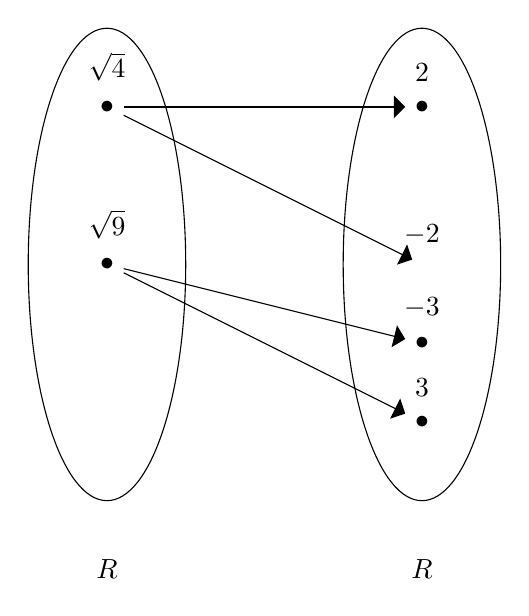
\begin{tikzpicture}
\tikzstyle{freccia} = [-triangle 90]
\draw  (0,0) node [label=$\sqrt{9}$] (v4) {$\bullet$} ellipse (1 and 3);
\draw  (4,0) node [label=$-2$](v3) {} ellipse (1 and 3);
\node[label=$\sqrt{4}$](v1) at (0,2) {$\bullet$};
%\node[label=$4$] (v5) at (0,-2) {$\bullet$};
\node[label=$2$] (v2) at (4,2) {$\bullet$};
\node[label=$3$] (v6) at (4,-2) {$\bullet$};
\node[label=$-3$] (v7) at (4,-1) {$\bullet$};
%\node[label=$-2$] (v8) at (0,1) {$\bullet$};
\node[label=below:$R$] at (0,-3.5) {};
\node[label=below:$R$]at (4,-3.5) {};
\draw[freccia] (v1) -- (v2);
\draw[freccia] (v1) -- (v3);
\draw [freccia](v4) -- (v7);
\draw [freccia](v4) -- (v6);
%\draw [freccia](v8) -- (v2);
\end{tikzpicture}
\end{document}